\pdfminorversion=4
\documentclass[aspectratio=169]{beamer}

\mode<presentation>
{
  \usetheme{default}
  \usecolortheme{default}
  \usefonttheme{default}
  \setbeamertemplate{navigation symbols}{}
  \setbeamertemplate{caption}[numbered]
  \setbeamertemplate{footline}[frame number]  % or "page number"
  \setbeamercolor{frametitle}{fg=white}
  \setbeamercolor{footline}{fg=black}
} 

\usepackage[english]{babel}
\usepackage[utf8x]{inputenc}
\usepackage{tikz}
\usepackage{courier}
\usepackage{array}
\usepackage{bold-extra}
\usepackage{minted}
\usepackage[thicklines]{cancel}
\usepackage{fancyvrb}

\xdefinecolor{dianablue}{rgb}{0.18,0.24,0.31}
\xdefinecolor{darkblue}{rgb}{0.1,0.1,0.7}
\xdefinecolor{darkgreen}{rgb}{0,0.5,0}
\xdefinecolor{darkgrey}{rgb}{0.35,0.35,0.35}
\xdefinecolor{darkorange}{rgb}{0.8,0.5,0}
\xdefinecolor{darkred}{rgb}{0.7,0,0}
\definecolor{darkgreen}{rgb}{0,0.6,0}
\definecolor{mauve}{rgb}{0.58,0,0.82}

\title[yyyy-mm-dd-DESCRIPTION]{TITLE}
\author{Jim Pivarski}
\institute{Princeton University -- IRIS-HEP}
\date{MONTH DAY, YEAR}

\usetikzlibrary{shapes.callouts}

\begin{document}

\logo{\pgfputat{\pgfxy(0.11, 7.4)}{\pgfbox[right,base]{\tikz{\filldraw[fill=dianablue, draw=none] (0 cm, 0 cm) rectangle (50 cm, 1 cm);}\mbox{\hspace{-8 cm}
\includegraphics[height=1 cm]{princeton-logo-long.png}\hspace{0.1 cm}\raisebox{0.1 cm}{
\includegraphics[height=0.8 cm]{iris-hep-logo-long.png}}\hspace{0.1 cm}}}}}

\begin{frame}
  \titlepage
\end{frame}

\logo{\pgfputat{\pgfxy(0.11, 7.4)}{\pgfbox[right,base]{\tikz{\filldraw[fill=dianablue, draw=none] (0 cm, 0 cm) rectangle (50 cm, 1 cm);}\mbox{\hspace{-8 cm}
\includegraphics[height=1 cm]{princeton-logo.png}\hspace{0.1 cm}\raisebox{0.1 cm}{
\includegraphics[height=0.8 cm]{iris-hep-logo.png}}\hspace{0.1 cm}}}}}

% Uncomment these lines for an automatically generated outline.
%\begin{frame}{Outline}
%  \tableofcontents
%\end{frame}

% START START START START START START START START START START START START START

\begin{frame}{First slide}
\vspace{0.5 cm}
HERE
\end{frame}

%% \begin{frame}[fragile]
%% \frametitle{Map-reduce}

%% Hadoop executes two sets of independent, identical processors:
%% \begin{itemize}
%% \item Mappers, which transform each input to a $\langle$key, value$\rangle$ pair.
%% \item Reducers, each operates on all values that have a given key.
%% \end{itemize}

%% \vspace{-0.1 cm}
%% \begin{columns}
%% \column{0.5\linewidth}
%% \begin{lstlisting}[frame=single]
%% def mapper($webpage$):
%%   for $word$ in $webpage$.split():
%%     yield ($word$, $webpage$)
%% $$
%% \end{lstlisting}
%% \column{0.58\linewidth}
%% \begin{lstlisting}[frame=single]
%% def reducer($word$, $webpages$):
%%   searchIndex[$word$] = {}
%%   for $webpage$ in $webpages$:
%%     searchIndex[$word$].add($webpage$)
%% \end{lstlisting}
%% \end{columns}

%% The system groups data by key in an optimized way (independent partial sorts followed by merge, minimizing network bandwidth).

%% \vspace{0.2 cm}
%% \mbox{ } \hfill 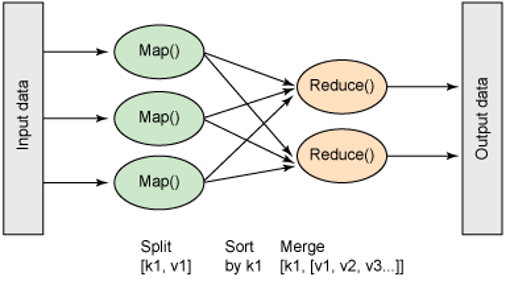
\includegraphics[width=0.6\linewidth]{PLOTS/mapreduce-diagram-by-ibm.png} \hfill \mbox{ }
%% \end{frame}

%% \begin{frame}[fragile]{Nested query in C++}
%% \vspace{0.5 cm}
%% {\bf Example query:}
%% \begin{center}
%% \begin{minipage}{0.95\linewidth}
%% \textcolor{darkblue}{``Momentum of the track with $|\eta|$ $<$ 2.4 that has the most hits.''}
%% \end{minipage}
%% \end{center}
%% \small
%% \begin{minted}{c++}
%% Track *best = NULL;
%% for (int i = 0;  i < tracks.size();  i++) {
%%   if (fabs(tracks[i]->eta) < 2.4)
%%     if (best == NULL ||
%%         tracks[i]->hits.size() > best->hits.size())
%%       best = tracks[i];
%% }
%% if (best != NULL)
%%   return best->pt;
%% else
%%   return 0.0;
%% \end{minted}
%% \end{frame}

%% \begin{frame}[fragile]{Nested query in SQL}
%% \vspace{0.5 cm}
%% {\bf Example query:}
%% \begin{center}
%% \begin{minipage}{0.95\linewidth}
%% \textcolor{darkblue}{``Momentum of the track with $|\eta|$ $<$ 2.4 that has the most hits.''}
%% \end{minipage}
%% \end{center}
%% \small
%% \begin{minted}{sql}
%% WITH hit_stats AS (
%%   SELECT hit.track_id, COUNT(*) AS hit_count FROM hit
%%     GROUP BY hit.track_id),
%%  track_sorted AS (
%%     SELECT track.*, 
%%     ROW_NUMBER() OVER (
%%      PARTITION BY track.event_id
%%      ORDER BY hit_stats.hit_count DESC)
%%   track_ordinal FROM track INNER JOIN hit_stats
%%     ON hit_stats.track_id = track.id
%%     WHERE ABS(track.eta) < 2.4)
%%  SELECT * FROM event INNER JOIN track_sorted
%%    ON track_sorted.event_id = event.id
%% WHERE
%%   track_sorted.track_ordinal = 1
%% \end{minted}
%% \end{frame}

\end{document}
